In this section, we will consider cluster structures of type $\dynBCFG$ and all standard affine type on $N$-graphs with certain symmetry.

Recall that if a quiver of type $\dynX$ is globally foldable with respect to the $G$-action, then the folded cluster pattern is of type $\dynY$.
We consider the triples $(\dynX, G, \dynY)$ shown in Table~\ref{table:foldings}.

\begin{table}[ht]
\[
\renewcommand\arraystretch{1.5}
\begin{array}{c|cccc}
\hline
\multirow{2}{*}{\text{rotation}}
&(\dynA_{2n-1},\Z/2\Z, \dynB_n)
&(\dynD_4,\Z/3\Z, \dynG_2)
&(\exdynE_6,\Z/3\Z, \exdynG_2)\\
%
&(\exdynD_{2n\ge6},\Z/2\Z, \exdynB_n)
&(\exdynD_4,\Z/2\Z, \exdynC_2)
%&(\exdynD_4,\Z/2\Z, \dynA_5^{(2)})
\\
\hline
%
\multirow{2}{*}{\text{conjugation}}
&(\dynD_{n+1},\Z/2\Z, \dynC_n)
&(\dynE_{6},\Z/2\Z, \dynF_4)\\
&(\exdynE_6,\Z/2\Z, \dynE_6^{(2)})
&(\exdynE_7,\Z/2\Z, \exdynF_4)
&(\exdynD_4,\Z/2\Z, \dynA_5^{(2)})\\
\hline
\end{array}
\]
\caption{Folding by rotation and conjugation}
\label{table:foldings}
\end{table}


\subsection{Group actions on \texorpdfstring{$N$}{N}-graphs}

For each triple $(\dynX, G, \dynY)$, we first consider the $G$-action on each $N$-graph of type $\dynX$.

\subsubsection{Rotation action}
Let $(\dynX, G, \dynY)$ be one of five cases in the first row of Table~\ref{table:foldings}.
We will denote the generator of $G=\Z/2\Z$ or $\Z/3\Z$ by $\tau$, which acts on $N$-graphs $\ngraph$ by $\pi$- or $2\pi/3$-rotation, respectively.

Notice that for each $\dynX=\dynA_{2n-1}, \dynD_4, \exdynE_6, \exdynD_{2n\ge6},$ or $\exdynD_4$, we may assume that the Legendrian $\legendrian(\dynX)$ in $J^1\sphere^1$ is invariant under the $\pi$-rotation since the braid $\beta(\dynX)$ representing $\legendrian(\dynX)$ has the rotation symmetry as follows:
\begin{align*}
\beta(\dynA_{2n-1})&=\left(\sigma_1^{n+1}\right)^2,&
\beta(\dynD_4) &=\left(\sigma_2\sigma_1^3\right)^3,&
\beta(\exdynE_6)&=\left(\sigma_2\sigma_1^4\right)^3,\\
\beta(\exdynD_{2n})&=\left(\sigma_2\sigma_1^3\sigma_2\sigma_1^3\sigma_2\sigma_3\sigma_1^{n-2}\right)^2,n\ge 3,&
\beta(\exdynD_4)&=\left(\sigma_2\sigma_1^3\sigma_2\sigma_1^3\sigma_2\sigma_3\right)^2.
\end{align*}

Now the generator $\tau$ acts on the set $\Ngraphs(\legendrian(\dynX))$ of equivalent classes of $N$-graphs with cycles whose boundary is precisely $\legendrian(\dynX)$.
Indeed, for each $(\ngraph, \nbasis)$ in $\Ngraphs(\legendrian(\dynX))$, we have
\[
\tau\cdot(\ngraph, \nbasis)=
\begin{cases}
R_\pi (\ngraph, \nbasis) & \text{ if }\tau\in \Z/2\Z;\\
R_{2\pi/3} (\ngraph, \nbasis) & \text{ if }\tau\in \Z/3\Z,
\end{cases}
\]
where $R_\theta$ is the induced action on $N$-graphs with cycles from the $\theta$-rotation on $\disk^2$. See Figure~\ref{figure:action on Ngraph of type A}.

\begin{figure}[ht]
\subfigure[$\Z/2\Z$-action on $(\ngraph, \nbasis)$\label{figure:action on Ngraph of type A}]{
\begin{tikzcd}[ampersand replacement=\&]
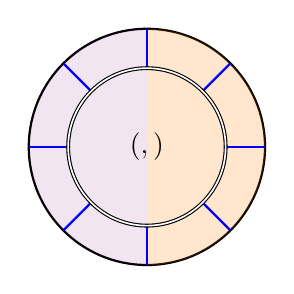
\begin{tikzpicture}[baseline=-.5ex, scale=0.5]
\draw[thick] (0,0) circle (3);
\fill[orange, opacity=0.2] (-90:3) arc(-90:90:3) -- cycle;
\fill[violet, opacity=0.1] (90:3) arc(90:270:3) -- cycle;
\foreach \i in {0,...,8} {
\draw[blue,thick] ({\i*45}:3) -- ({\i*45}:2);
}
\draw[double] (0,0) node {$(\ngraph,\nbasis)$} circle (2);
\end{tikzpicture}
\arrow[r,"\tau",yshift=.5ex]\&
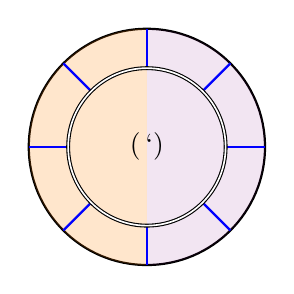
\begin{tikzpicture}[baseline=-.5ex, scale=0.5]
\draw[thick] (0,0) circle (3);
\fill[violet, opacity=0.1] (90:3) arc(90:-90:3) -- cycle;
\fill[orange, opacity=0.2] (-90:3) arc(-90:-270:3) -- cycle;
\foreach \i in {0,...,8} {
\draw[blue,thick] ({\i*45}:3) -- ({\i*45}:2);
}
\draw[double] (0,0) node[rotate=180] {$(\ngraph,\nbasis)$} circle (2);
\end{tikzpicture}
\arrow[l, "\tau", yshift=-.5ex]
\end{tikzcd}
}

\subfigure[$\Z/3\Z$-action on $(\ngraph, \nbasis)$]{
\begin{tikzcd}[ampersand replacement=\&]
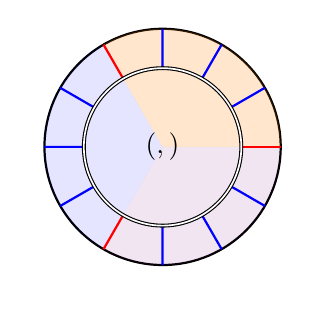
\begin{tikzpicture}[baseline=-.5ex, scale=0.5]
\draw[thick] (0,0) circle (3);
\fill[orange, opacity=0.2] (0,0) -- (0:3) arc(0:120:3) -- cycle;
\fill[violet, opacity=0.1] (0,0) -- (-120:3) arc(-120:0:3) -- cycle;
\fill[blue, opacity=0.1] (0,0) -- (120:3) arc (120:240:3) -- cycle;
\foreach \i in {0, 120, 240} {
\begin{scope}[rotate=\i]
\draw[blue, thick] (30:3) -- (30:2) (60:3) -- (60:2) (90:3) -- (90:2);
\draw[red, thick] (0:3) -- (0:2);
\end{scope}
}
\draw[double] (0,0) node {$(\ngraph,\nbasis)$} circle (2);
\end{tikzpicture}
\arrow[r,"\tau"]\&
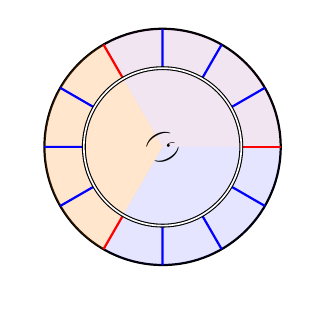
\begin{tikzpicture}[baseline=-.5ex, scale=0.5]
\draw[thick] (0,0) circle (3);
\fill[orange, opacity=0.2] (0,0) -- (120:3) arc(120:240:3) -- cycle;
\fill[violet, opacity=0.1] (0,0) -- (0:3) arc(0:120:3) -- cycle;
\fill[blue, opacity=0.1] (0,0) -- (-120:3) arc (-120:0:3) -- cycle;
\foreach \i in {0, 120, 240} {
	\begin{scope}[rotate=\i]
	\draw[blue, thick] (30:3) -- (30:2) (60:3) -- (60:2) (90:3) -- (90:2);
	\draw[red, thick] (0:3) -- (0:2);
	\end{scope}
}
\draw[double] (0,0) node[rotate=120] {$(\ngraph,\nbasis)$} circle (2);
\end{tikzpicture}
\arrow[r,"\tau"]\&
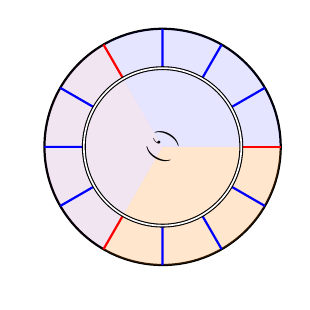
\begin{tikzpicture}[baseline=-.5ex, scale=0.5]
\draw[thick] (0,0) circle (3);
\fill[orange, opacity=0.2] (0,0) -- (-120:3) arc(-120:0:3) -- cycle;
\fill[violet, opacity=0.1] (0,0) -- (120:3) arc(120:240:3) -- cycle;
\fill[blue, opacity=0.1] (0,0) -- (0:3) arc (0:120:3) -- cycle;
\foreach \i in {0, 120, 240} {
\begin{scope}[rotate=\i]
\draw[blue, thick] (30:3) -- (30:2) (60:3) -- (60:2) (90:3) -- (90:2);
\draw[red, thick] (0:3) -- (0:2);
\end{scope}
}
\draw[double] (0,0) node[rotate=-120] {$(\ngraph,\nbasis)$} circle (2);
\end{tikzpicture}
\arrow[ll,"\tau", bend left=35]
\end{tikzcd}
}
\caption{Rotation actions on $N$-graphs}
\label{figure:rotation action}
\end{figure}


\subsubsection{Conjugation action}
Assume that $(\dynX, G, \dynY)$ is one of five cases in the second row of Table~\ref{table:foldings}.
We denote the generator for $G=\Z/2\Z$ by $\eta$.
Then, as before, the Legendrian $\tilde\legendrian(\dynX)$ is represented by the braid $\tilde\beta(\dynX)$ which is invariant under the conjugation as follows:
\begin{align*}
\tilde\beta(\dynD_{n+1})&=\sigma_2^n \sigma_{1,3}\sigma_2\sigma_{1,3}^3 \sigma_2\sigma_{1,3}\sigma_2^2\sigma_{1,3},&
\tilde\beta(\dynE_6)&=\sigma_2^3 \sigma_{1,3}\sigma_2\sigma_{1,3}^4 \sigma_2\sigma_{1,3}\sigma_2^2\sigma_{1,3},\\
\tilde\beta(\exdynE_6)&=\sigma_2^4 \sigma_{1,3}\sigma_2\sigma_{1,3}^4 \sigma_2\sigma_{1,3}\sigma_2^2\sigma_{1,3},&
\tilde\beta(\exdynE_7)&=\sigma_2^3 \sigma_{1,3}\sigma_2\sigma_{1,3}^5 \sigma_2\sigma_{1,3}\sigma_2^2\sigma_{1,3},&
\tilde\beta(\exdynD_4)&=(\sigma_2\sigma_{1,3}\sigma_2\sigma_{1,3}^2)^2.
\end{align*}

Therefore, the generator $\eta$ acts on the set $\Ngraphs(\tilde\legendrian(\dynX))$ by conjugation.
That is, for each $(\ngraph, \nbasis)\in\Ngraphs(\tilde\legendrian(\dynX))$, we have
\[
\eta\cdot (\ngraph, \nbasis) = \overline{(\ngraph, \nbasis)}.
\]

\begin{remark}
One may consider the conjugation invariant degenerate $N$-graph $\tilde\ngraph(\dynA_{2n-1})$ instead of the rotation invariant $N$-graph $\ngraph(\dynA_{2n-1})$ as seen earlier in Remark~\ref{remark:degenerated Ngraph of type A}. 
Then it can be checked that these two actions are identical.
\end{remark}

\begin{remark}
The denegerated $N$-graph $\tilde\ngraph(\exdynD_4)$ admits the $\pi$-rotation action as well, which is essentially equivalent to the conjugation action on $\tilde\ngraph(\exdynD_4)$. We omit the detail.
\end{remark}


\subsection{Invariant \texorpdfstring{$N$}{N}-graphs and Lagrangian fillings}
Throughout this section, we assume that $(\dynX, G, \dynY)$ is one of the triples in Table~\ref{table:foldings}.
For an $N$-graph $\ngraph$ in $\Ngraphs(\legendrian(\dynX))$ or  $\Ngraphs(\tilde\legendrian(\dynX))$, we say that $(\ngraph, \nbasis)$ is \emph{$G$-invariant} if for each $g\in G$,
\[
g\cdot(\ngraph, \nbasis) = (\ngraph, \nbasis).
\]
Namely,
\begin{enumerate}
\item the $N$-graph $\ngraph$ is invariant under the action of $g$,
\item the sets of cycles $\nbasis$ and $g(\nbasis)$ are identical up to relabeling $\cycle \leftrightarrow g(\cycle)$ for $\cycle\in\nbasis$.
\end{enumerate}

The following statements are obvious but important observations.
\begin{lemma}\label{lemma:Lagrangian fillings with symmetry}
For a free $N$-graph $\ngraph$, let
\[
L(\ngraph)\colonequals(\pi\circ\iota)(\Legendrian(\ngraph))
\]
be the Langrangian surface defined by $\ngraph$ in $\mathbb{C}^2$.
\begin{enumerate}
\item If $\ngraph$ is invariant under the $\theta$-rotation, then $L(\ngraph)$ is invariant under the $\theta$-rotation in $\mathbb{C}^2$
\[
(z_1,z_2)\mapsto (z_1\cos(\theta) +z_2\sin(\theta), -z_1\sin(\theta)+z_2\cos(\theta)).
\]
\item If $\ngraph$ is invariant under the conjugation, then $L(\ngraph)$ is invariant under the antisymplectic involution in $\mathbb{C}^2$
\[
(z_1,z_2)\mapsto (\bar z_1, \bar z_2).
\]
\end{enumerate}
\end{lemma}

\begin{lemma}\label{lemma:initial Ngraphs are G-invariant}
The $N$-graphs $\ngraph(\dynX)$ for $\dynX=\dynA_{2n-1}, \dynD_4, \exdynE_6, \exdynD_{2n\ge 6}, \exdynD_4$ and the degenerate $N$-graphs $\tilde\ngraph(\dynX)$ for $\dynX=\dynD_{n+1}, \dynE_6, \exdynE_6, \exdynE_7, \exdynD_4$ are all invariant under the $G$-action.
\end{lemma}

%\begin{lemma}\label{lemma:coxeter padding is invariant}
%The Coxeter paddings $\coxeterpadding(\dynX)$ for $\dynX=\dynA_{2n-1}, \dynD_4, \exdynE_6, \exdynD_{2n\ge6}$ and $\exdynD_4$ are invariant under $\pi$- or $2\pi/3$-rotation.
%\end{lemma}


\begin{lemma}\label{lemma:mutation preserves invariance}
Suppose that $g\in G$ acts on $(\ngraph, \nbasis)$.
If the Legendrian mutation $\mutation_{\cycle}(\ngraph, \nbasis)$ is realizable, then
\[
\mutation_{g(\cycle)}\left(g\cdot(\ngraph,\nbasis)\right) = g\cdot\left(\mutation_{\cycle}(\ngraph,\nbasis)\right).
\]
In particular, for a $G$-orbit $I\subset\nbasis$ consists of pairwise disjoint cycles, if $(\ngraph,\nbasis)$ is $G$-invariant and the Legendrian orbit mutation $\mutation_{I}(\ngraph,\nbasis)$ is realizable, then $\mutation_I(\ngraph,\nbasis)$ is $G$-invariant as well.
\end{lemma}


On the other hand, if we have a $G$-invariant $N$-graph $(\ngraph, \nbasis)$ with cycles, it gives us a $G$-admissible quiver $\quiver(\ngraph, \nbasis)$.
\begin{lemma}\label{lemma:G-invariant Ngraphs imply G-admissible quivers}
Let $(\ngraph, \nbasis)$ be a $G$-invariant $N$-graph with cycles.
Then the quiver $\quiver(\ngraph, \nbasis)$ is $G$-admissible.
\end{lemma}
\begin{proof}
By definition of $G$-invariance of $(\ngraph, \nbasis)$, it is obvious that the quiver $\quiver=\quiver(\ngraph, \nbasis)$ is $G$-invariant.
On the other hand, since $\dynX$ is either a finite or an affine Dynkin diagram, the $G$-invariance of the quiver $\quiver$ implies the $G$-admissibility of $\quiver$  by Theorem~\ref{thm_invariant_seeds_form_folded_pattern}.
\end{proof}

\begin{proposition}\label{proposition:G-invariant Ngraphs}
For each $Y$-seed $(\bfy',\qbasispr')$ of type $\dynY$, there exists a $G$-invariant $N$-graph with cycles $(\ngraph, \nbasis)$ of type $\dynX$ such that
\[
\Psi(\ngraph, \nbasis)^G = (\bfy',\qbasispr').
\]
\end{proposition}
\begin{proof}
For each $\dynX$, let $(\ngraph_{t_0},\nbasis_{t_0})$ be the $N$-graph with cycles defined as follows:
\begin{align*}
(\ngraph_{t_0},\nbasis_{t_0}) \colonequals
\begin{cases}
(\ngraph(\dynX),\nbasis(\dynX)) & \text{ if } \dynX=\dynA_{2n-1}, \dynD_4, \exdynE_6, \exdynD_{2n\ge 6}, \exdynD_4, G\text{ acts as rotation};\\
(\tilde\ngraph(\dynX),\tilde\nbasis(\dynX)) & \text{ if } \dynX=\dynD_{n+1}, \dynE_6, \exdynE_6, \exdynE_7, \exdynD_4, G\text{ acts as conjugation}.
\end{cases}
\end{align*}

We regard the $Y$-seed defined by $(\ngraph_{t_0},\nbasis_{t_0})$ as the intial seed $(\bfy_{t_0}, \qbasispr_{t_0})$
\[
(\bfy_{t_0}, \qbasispr_{t_0})=\Psi(\ngraph_{t_0},\nbasis_{t_0}).
\]
As seen in Lemmas~\ref{lemma:initial Ngraphs are G-invariant} and \ref{lemma:G-invariant Ngraphs imply G-admissible quivers},  $(\ngraph_{t_0},\nbasis_{t_0})$ is $G$-invariant and so is the quiver $\quiver(\ngraph_{t_0},\nbasis_{t_0})$.
Therefore, we have the folded seed $(\bfy_{t_0}, \qbasispr_{t_0})^G$ which plays the role of the initial seed of the $Y$-pattern of type~$\dynY$.

Let $(\bfy', \qbasispr')$ be an $Y$-seed of the $Y$-pattern of type $\dynY$.
By Lemma~\ref{lemma:normal form}, there exist $r\in \Z$ and a sequence of mutations $\mutation_{j_1}^\dynY, \dots, \mutation_{j_L}^\dynY$ such that 
\[
(\bfy', \qbasispr') = (\mutation_{j_L}^\dynY\cdots\mutation_{j_1}^\dynY)
((\mutation_\quiver^\dynY)^r((\bfy_{t_0}, \qbasispr_{t_0})^G)).
\]
Moreover, the indices $j_1,\dots, j_L$ misses at least one index, say $i$.

Then Theorem~\ref{thm_invariant_seeds_form_folded_pattern} implies the existence of the $G$-admissible $Y$-seed $(\bfy, \qbasispr)$ of type $\dynX$ such that $(\bfy,\qbasispr)^G=(\bfy',\qbasispr')$ and
\[
(\bfy,\qbasispr) = (\mutation_{I_L}^\dynX\cdots\mutation_{I_1}^\dynX)
((\mutation_\quiver^\dynX)^r(\bfy_{t_0},\qbasispr_{t_0})),
\]
where $I_k$ is $G$-orbit corresponding to $j_k$ for each $1\le k\le L$.
It suffices to prove that the $N$-graph
\[
(\ngraph, \nbasis)=(\mutation_{I_L}\cdots\mutation_{I_1})((\ncoxeter)^r(\ngraph_{t_0},\nbasis_{t_0}))
\]
is well-defined and $G$-invariant so that $(\bfy, \qbasispr)=\Psi(\ngraph,\nbasis)$ is $G$-admissible by Proposition~\ref{proposition:equivariance of mutations} as desired.

By Lemma~\ref{lemma:Legendriam Coxeter mutation of type An}, Propositions~\ref{proposition:effect of Legendrian Coxeter mutation}, \ref{proposition:coxeter realization D-type} and \ref{proposition:coxeter realization denegerate type}, the Legendrian Coxeter mutation $\ncoxeter^r(\ngraph_{t_0}, \nbasis_{t_0})$ is realizable so that
\[
\Psi(\ncoxeter^r(\ngraph_{t_0}, \nbasis_{t_0}))
=(\mutation_\quiver)^r(\bfy_{t_0},\qbasispr_{t_0}).
\]

Since $\ncoxeter^r(\ngraph_{t_0}, \nbasis_{t_0})$ is the concatenation of Coxeter paddings on the initial $N$-graph $(\ngraph_{t_0},\nbasis_{t_0})$, it suffices to prove that the Legendrian mutation
$(\mutation_{I_L}\cdots\mutation_{I_1})(\ncoxeter^r(\ngraph_{t_0}, \nbasis_{t_0}))$
is realizable, which is equivalent to the realizability of
$(\mutation_{I_L}\cdots\mutation_{I_1})(\ngraph_{t_0}, \nbasis_{t_0})$.

On the other hand, since the indices $j_1,\dots, j_L$ misses the index $i$, the orbits $I_1,\dots, I_L$ misses one orbit $I$ corresponding to $i$.
In other words, the sequence of mutations $\mutation_{I_1},\dots,\mutation_{I_L}$ can be performed inside the subgraph of the exchange graph $\exchange(\Roots(\dynX))$, which is isomorphic to $\exchange(\Roots(\dynX \setminus I))$.
Then the root system $\Roots(\dynX\setminus I)$ is decomposed into $\Roots(\dynX^{(1)}), \dots, \Roots(\dynX^{(\ell)})$, where $\dynX\setminus I = \dynX^{(1)}\cup\cdots\cup\dynX^{(\ell)}$.
Moreover, the sequence of mutations $\mutation_{I_1},\dots,\mutation_{I_L}$ can be decomposed into sequences $\mutation^{(1)},\dots, \mutation^{(\ell)}$ of mutations on $\dynX^{(1)},\dots,\dynX^{(\ell)}$.

Similarly, we may decompose the $N$-graph $(\ngraph_{t_0}, \nbasis_{t_0})$ into $N$-subgraphs 
\[
(\ngraph^{(1)}, \nbasis^{(1)}),\dots,(\ngraph^{(\ell)}, \nbasis^{(\ell)})
\]
along cycles in $I\subset\nbasis_{t_0}$ as done in the previous section.
Then the Legendrian mutation $(\mutation_{I_L}\cdots\mutation_{I_1})(\ngraph_{t_0},\nbasis_{t_0})$ is realizable if and only if so is $\mutation^{(j)}(\ngraph^{(j)},\nbasis^{(j)})$ for each $1\le j\le \ell$.
This can be done by induction on rank of the root system and so the $N$-graph $(\ngraph, \nbasis)$ with $\Psi(\ngraph,\nbasis)=(\bfy,\qbasispr)$ is well-defined.

Finally, the $G$-invariance of $(\ngraph, \nbasis)$ follows from Lemma~\ref{lemma:mutation preserves invariance}.
\end{proof}


\begin{theorem}[Folding of $N$-graphs]\label{thm:folding of N-graphs}
The following holds:
\begin{enumerate}
\item The Legendrian $\lambda(\dynA_{2n-1})$ has $\binom{2n}{n}$ Lagrangian fillings which are invariant under the $\pi$-rotation and  admit the $Y$-pattern of type $\dynB_n$.
\item The Legendrian $\lambda(\dynD_{4})$ has $8$ Lagrangian fillings which are invariant under the $2\pi/3$-rotation and admit the $Y$-pattern of type $\dynG_2$.
\item The Legendrian $\lambda(\exdynE_{6})$ has Lagrangian fillings which are invariant under the $2\pi/3$-rotation and admit the $Y$-pattern of type $\exdynG_2$.
\item The Legendrian $\lambda(\exdynD_{2n})$ with $n\ge 3$ has Lagrangian fillings which are invariant under the $\pi$-rotation and admit the $Y$-pattern of type $\exdynB_n$.
\item The Legendrian $\lambda(\exdynD_4)$ has Lagrangian fillings which are invariant under the $\pi$-rotation and admit the $Y$-pattern of type $\exdynC_2$.
%
\item The Legendrian $\tilde\lambda(\dynE_{6})$ has $105$ Lagrangian fillings which are invariant under the antisymplectic involution and admit the $Y$-pattern of type $\dynF_4$.
\item The Legendrian $\tilde\lambda(\dynD_{n+1})$ has $\binom{2n}{n}$ Lagrangian fillings which are invariant under the antisymplectic involution and admit the $Y$-pattern of type $\dynC_n$.
\item The Legendrian $\tilde\lambda(\exdynE_{6})$ has Lagrangian fillings which are invariant under the antisymplectic involution and admit the $Y$-pattern of type $\dynE_6^{(2)}$.
\item The Legendrian $\tilde\lambda(\exdynE_{7})$ has Lagrangian fillings which are invariant under the antisymplectic involution and admit the $Y$-pattern of type $\exdynF_4$.
\item The Legendrian $\tilde\lambda(\exdynD_4)$ has Lagrangian fillings which are invariant under the antisymplectic involution and admit the $Y$-pattern of type $\dynA_5^{(2)}$.
\end{enumerate}
\end{theorem}
\begin{proof}
Let $(\dynX, G,\dynY)$ be one of the triples in Table~\ref{table:foldings}.
By Proposition~\ref{proposition:G-invariant Ngraphs}, each $Y$-seed of the $Y$-pattern of type $\dynY$ is realizable by a $G$-invariant $N$-graph, which gives us a Lagrangian filling with a certain symmetry by Lemma~\ref{lemma:Lagrangian fillings with symmetry}.
This completes the proof.
\end{proof}
